\section[Problem 4]{Problem 4: Hazard--Exposure--Response Assessment on Settlement Catchments}
\label{sec:q4}

\subsection{Assessment Units}

Township boundaries of Hengzhou are not publicly available, and the 17 towns are too few for objective weighting or for a meaningful relief model. We take as units the Voronoi cells of all 393 OSM settlement nodes (370 villages, 16 towns, 5 hamlets, one city node and one suburb), clipped to the city boundary. A cell is the area that is closer to its settlement than to any other, i.e. the natural catchment that relief for that settlement would serve. The cells partition the boundary exactly (sum 3440.0919\,km$^2$ against 3440.0920\,km$^2$), and the new inundation of the units sums to the city value of Problem~3 (26.9025\,km$^2$, relative difference $4\times10^{-9}$). Each unit inherits the town or city zone of its nearest town or city node, which gives 17 zones for reporting. A unit counts as affected if $A_{new,j}$ is at least one minimum mapping unit, 0.005\,km$^2$. 259 of the 393 units are affected, and only these are scored.

\subsection{Indicator System}

The core indicators are newly inundated area, proportion and intensity; exposure of people and critical facilities enters as the fourth. Every indicator in Table~\ref{tab:q4_ind} is an overlay of the Problem~3 raster $F_{0716}$ with a public layer; the assessment changes whenever $F$ changes. All indicators are oriented so that larger means worse.

\begin{table}[!ht]
\centering
\caption{Indicators of the regional assessment}
\label{tab:q4_ind}
\small
\begin{tabular}{p{0.13\textwidth}p{0.28\textwidth}p{0.35\textwidth}p{0.11\textwidth}}
\toprule
Criterion & Indicator & Definition & Weight \\
\midrule
Hazard & H1 new area $A_{new,j}$ (km$^2$) & $\sum_{p\in F\cap j}a_p$ & 0.233 \\
 & H2 proportion $\rho_j$ & $A_{new,j}/A_{reg,j}$ & 0.198 \\
 & H3 intensity $I_j$ & expected grade $\sum_g g\,\pi_{jg}$ by \eqref{eq:grade_mc} & 0.108 \\
Exposure & E1 flooded population & $\sum_c \mathrm{pop}_c\,\phi_c$, $\phi_c$ flooded share of 100\,m cell $c$ & 0.055 \\
 & E2 flooded built-up (km$^2$) & $|F\cap\{\mathrm{WC}=50\}|_a$ & 0.055 \\
 & E3 flooded cropland (km$^2$) & $|F\cap\{\mathrm{WC}=40\}|_a$ & 0.047 \\
 & E4 exposed facilities & facility proxies within 500\,m of $F$ & 0.140 \\
Response & R1 access time (min) & flood-cut network time from the flooded-population centroid to the nearest unflooded facility proxy & 0.080 \\
 & R2 road-cut share & impassable road length / road length in the unit & 0.084 \\
\bottomrule
\end{tabular}
\end{table}

Terrain enters through the REM guard inside $F$. Built-up land is taken from WorldCover because OSM holds only 609 building footprints. Hospitals and shelters are represented by the facility proxies of Assumption~5 (town and city nodes plus schools), because OSM lists only five service points. A road edge is impassable if any of its sample points, taken every 20\,m, lies within 20\,m of $F$. Unreachable units get twice the largest finite access time, 165.6\,min. Over the whole city the overlay finds 13,954 flooded people, 1.88\,km$^2$ of flooded built-up land, 13.60\,km$^2$ of flooded cropland, 8 of 22 facility proxies within 500\,m of new inundation, and 117.4 of 2542.3\,km of roads cut. 75 affected units have no road path to an unflooded facility.

At 1\,km the two fields separate rather than co-vary (Fig.~\ref{fig:q4_grid1km}). Across the 1010 cells that carry new inundation the rank correlation of water area with resident population is $\rho_S=0.36$; the ten cells with the largest area hold 8.2\% of the flooded population, and the ten that hold the most people carry 4.9\% of the new water. A cell can be nearly dry and still shelter several hundred people; exposure is not a rescaling of the flood map, and the exposure criterion carries its own population and facility indicators instead of weighting area alone. Panels (A) and (B) of Fig.~\ref{fig:q4_grid1km} map the two fields and panel (C) their joint distribution, with the ten largest areas and the ten most populated cells ringed.

\begin{figure}[!ht]
  \centering
  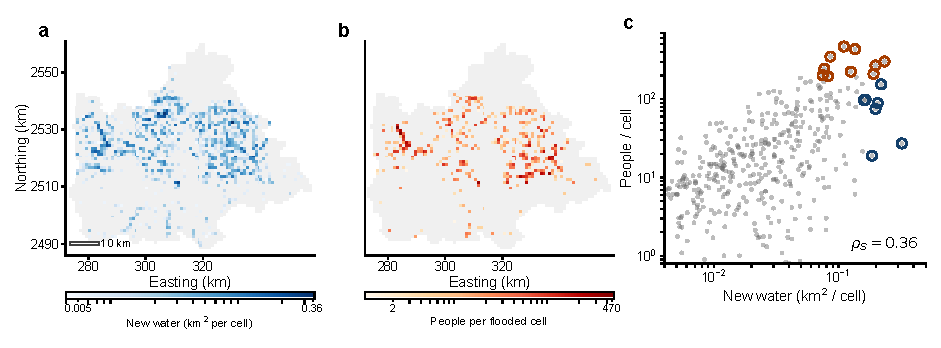
\includegraphics[width=0.90\textwidth,keepaspectratio]{../figures/fig_q4_grid1km.pdf}
  \caption{A 1\,km exposure layer over the mapped new inundation}
  \label{fig:q4_grid1km}
\end{figure}

\subsection{Combined Weights and the TOPSIS Index}

Indicators are min--max normalized over units, $r_{jk}=(X_{jk}-\min_jX_{jk})/(\max_jX_{jk}-\min_jX_{jk})$. Inside each criterion two objective weightings are combined. Entropy weights $w^e_k\propto1-e_k$ with $e_k=-\frac{1}{\ln n}\sum_j\tilde r_{jk}\ln\tilde r_{jk}$ and $\tilde r_{jk}=r_{jk}/\sum_jr_{jk}$ reward discrimination between units. CRITIC weights~\cite{diakoulaki1995critic} $w^c_k\propto s_k\sum_l(1-\mathrm{corr}_{kl})$ reward variation that is not redundant. The game-theoretic combination chooses the mix closest to both:
\begin{equation}
\begin{bmatrix}w^e\!\cdot\!w^e & w^e\!\cdot\!w^c\\ w^c\!\cdot\!w^e & w^c\!\cdot\!w^c\end{bmatrix}
\begin{bmatrix}\alpha_1\\ \alpha_2\end{bmatrix}=
\begin{bmatrix}w^e\!\cdot\!w^e\\ w^c\!\cdot\!w^c\end{bmatrix},\qquad
w^{(c)}=\frac{|\alpha_1|w^e+|\alpha_2|w^c}{|\alpha_1|+|\alpha_2|}.
\label{eq:game_weights}
\end{equation}
For the hazard criterion, entropy gives (0.477, 0.404, 0.119) and CRITIC (0.320, 0.273, 0.407), and the combination with $\alpha=(0.767,0.303)$ gives (0.432, 0.367, 0.201). Between criteria we use a judgment that follows the problem text, hazard as core, exposure second, response third, through the AHP matrix
\begin{equation}
J=\begin{bmatrix}1&2&3\\ 1/2&1&2\\ 1/3&1/2&1\end{bmatrix},\qquad
\Omega=\text{principal eigenvector of }J,\qquad
\mathrm{CR}=\frac{(\lambda_{max}-3)/2}{0.58},
\label{eq:ahp}
\end{equation}
which gives $\Omega=(0.540,0.297,0.163)$ with $\lambda_{max}=3.0092$ and $\mathrm{CR}=0.0079<0.1$. The final weights $w_k=\Omega_{c(k)}w^{(c(k))}_k$ sum to one and are listed in Table~\ref{tab:q4_ind}. The three core hazard indicators carry 0.539 of the total weight. The disaster index is the TOPSIS closeness on $v_{jk}=w_kr_{jk}$,
\begin{equation}
S_j=\frac{D^-_j}{D^+_j+D^-_j},\qquad D^\pm_j=\big\lVert v_j-v^\pm\big\rVert_2,\qquad v^+_k=\max_jv_{jk},\ v^-_k=\min_jv_{jk},
\label{eq:topsis}
\end{equation}
so $S_j=1$ for a unit at the worst observed value of every indicator. Four disaster levels (I most severe) are formed by Jenks natural breaks of $S_j$. Zones are scored analogously from aggregated indicators.

\subsection{Spatial Pattern of Disaster Severity}

Levels hold 3 units in Level~I, 28 in Level~II, 96 in Level~III and 132 in Level~IV. Whether severity follows the flood alone, or exposure reorders it, is visible in Fig.~\ref{fig:q4_risk_map}, a bivariate map crossing hazard ($H_1$) with exposure ($E_1$), each split at the tertiles of the affected units.

\begin{figure}[!ht]
  \centering
  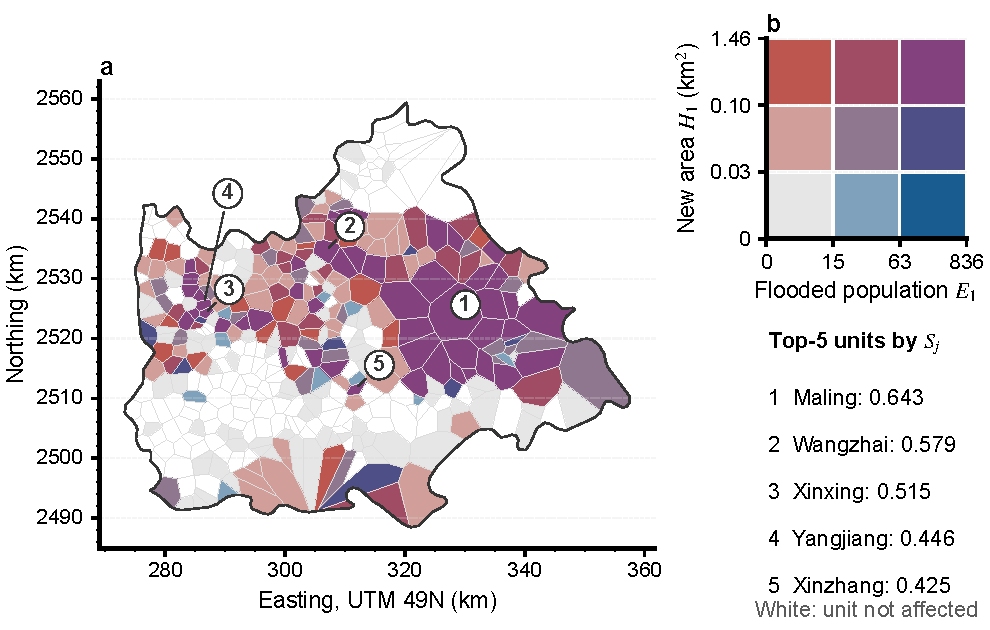
\includegraphics[width=0.90\textwidth,keepaspectratio]{../figures/fig_q4_risk_map.pdf}
  \caption{Hazard--exposure map of the 393 units}
  \label{fig:q4_risk_map}
\end{figure}

One belt carries the disaster: between northings 2520 and 2535\,km lie 16.78 of the 26.90\,km$^2$ of new inundation and 8298 of the 13,954 flooded people, with the Luancheng, Shitang, Maling and Yunbiao zones; south of northing 2505\,km, 56 units share 1.15\,km$^2$ and 237 people. Five catchments stand out: Maling town ($S=0.643$; 1.46\,km$^2$; 836 people; an exposed facility; no road access to an unflooded one), Wangzhai in the Shitang zone ($0.579$; 118 people; 9.2\% of its area newly wet), Xinxing ($0.515$) and Yangjiang ($0.446$) in Luancheng (13.2\% and 9.0\%), and Xinzhang in Liantang ($0.425$).

At zone level Shitang ranks first ($S=0.787$; 4.91\,km$^2$, 1189 people), then Maling (0.760; 2.96\,km$^2$, 2305 people), Luancheng (0.740; 3.58\,km$^2$, 2144 people), Yunbiao (0.648), Xiaoyi (0.558) and Nayang (0.501), all with flood shares of only 1.1--2.4\%. These are zone-level shares, not the city-level thresholds of Table~\ref{tab:grade_thr}: on a 243\,km$^2$ zone the same share means a tenth of the absolute area it does over the 3440\,km$^2$ city, and the four levels come from the Jenks breaks of $S_j$, not from the intensity table. Where the flood meets people and cut roads drives the ranking, not large flooded areas.

A stricter test grades on the other dimension: replacing the share $\rho_j$ with the absolute area $A_{new,j}$ -- a four-component Gaussian mixture on $\log_{10}A_{new,j}$ with boundaries 4.83, 9.32 and 21.39\,km$^2$ -- lifts 16 of the 259 affected units by one level, lowers none, and touches 433.4\,km$^2$ of the city. Spearman between the two gradings is 0.973; grading on area alone drops it to 0.749. What gets rewritten are the large-but-thin units a share-only rule understates, so the level assignment is stable to which dimension of the hazard is graded.

\subsection{Robustness of the Ranking}

A ranking used for relief must not depend on a particular weight vector. We draw $M=2000$ weight sets with $\Omega\sim\mathrm{Dir}(50\,\Omega_0)$ and $w^{(c)}\sim\mathrm{Dir}(50\,w^{(c)}_0)$ around the baseline, recompute the ranking each time, and compare it with rankings from hazard indicators only and from alternative Problem~3 inputs. Fig.~\ref{fig:q4_rank_robustness} summarizes the outcome.

\begin{figure}[!ht]
  \centering
  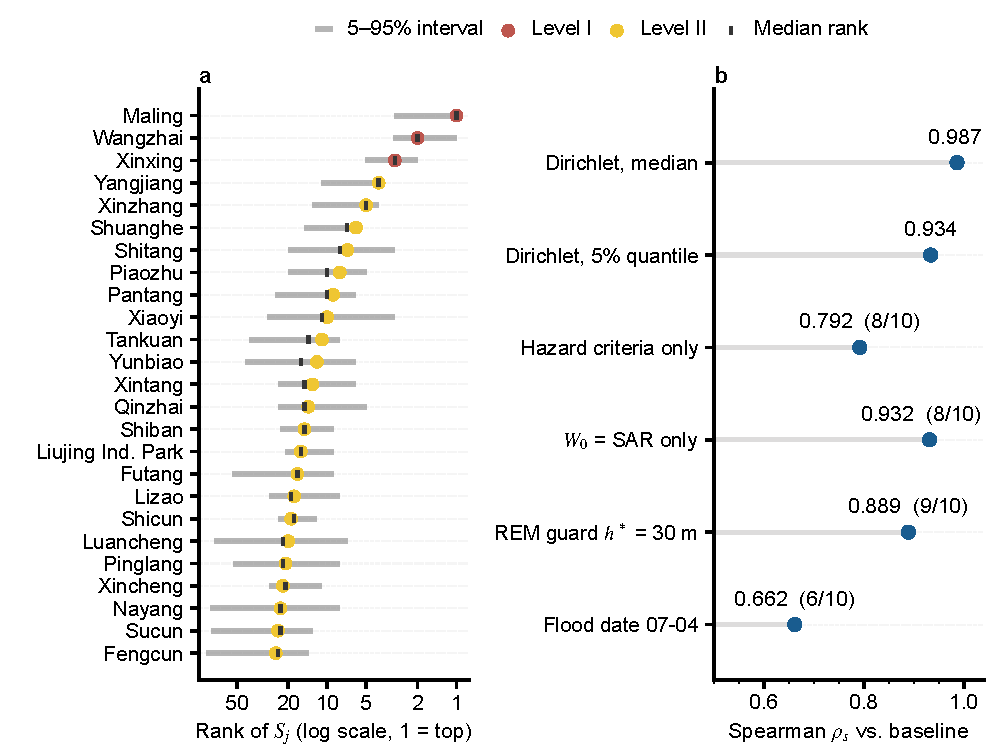
\includegraphics[width=0.90\textwidth,keepaspectratio]{../figures/fig_q4_rank_robustness.pdf}
  \caption{Robustness of the unit ranking}
  \label{fig:q4_rank_robustness}
\end{figure}

Weight perturbation leaves the ranking essentially unchanged: median Spearman against the baseline is 0.987, its 5\% quantile 0.934, and the 5--95\% rank intervals of the top units in panel (A) are narrow. Ranking by hazard alone gives 0.792 and keeps 8 of the top 10; exposure and response reorder about a fifth of the ranking, which is why they are there. Input data matter more than weights. With the 4 July flood the correlation falls to 0.662, while the SAR-only $W_0$ and the 30\,m guard leave it at 0.932 and 0.889 (Table~\ref{tab:sens_chain}). The ranking is a statement about the 16 July observation, and the letter turns that into a recommendation to recompute it after each pass\cite{deepseek2026,qwen2026,doubao2026}.
